\chapter{Related Work and Theory}
Inverse kinematics is applied in various fields, mainly robotics and computer
graphics. However, it is applied to a few unique problems, such as the
prediction of protein structure \cite{ccd_protein}. It has also found its uses in
rehabilitation medicine due to its biomechanical modelling ability. Over time,
many approaches have surfaced in order to solve the IK problem. There are
multiple families of solutions \cite{Aristidou2011} which suit different use
cases. Among others, trigonometric solutions can be used to solve certain IK
problems analytically \cite{raheem_trig}, however, these solutions are often limited to solving two
bone IK scenarios. More recently neural networks have also been used as a tool
to solve IK problems \cite{nn_IK}. This paper will go over the iterative and
heuristic approaches which provide less complex solutions when increasing the
kinematic chain length and degrees of freedom.

\section{Kinematics}
Kinematics is a branch of classical mechanics
concerned with the geometrically possible motion of a body or system of bodies
without consideration of the forces involved \cite{kinematics_britannica}.
A kinematic chain is a tree like hierarchical structure of joint transforms
which are connected to each other. Because the relationship between joints is
hierarchical, a transformation which is applied to a given joint affects all of
its descendant nodes. When manipulating a kinematic chain, transformations in
the form of rotations and translations are applied to joint transforms in order
to achieve a desired position of one or multiple transforms called the end
effectors. The problem of kinematics can be subdivided into two approaches which
each present their own problem and solution.

\begin{itemize}
    \item The problem of \textit{Forward Kinematics} which has to do with the
        identification of the final position of an end effector as a result of
        a set of transformations being applied to the kinematic chain to which
        the end effector belongs.
    \item The problem of \textit{Inverse Kinematics} which pertains to the
        search for a configuration of joint transformations for a kinematic
        chain which allow the end effector to reach a predefined target
        position.
\end{itemize}

The forward kinematics (FK) problem can be said to have a guaranteed solution as
long as the set of joint transformations used as an input are known. To solve
the FK problem, the transformations are applied to the kinematic chain, and the
transform of the end effector is taken as an output. On the contrary, when
dealing with IK, the given problem may have no solutions, one solution, or many
solutions. \\

\noindent\textit{No Solutions}

An IK problem with no solutions can occur for several reasons. Most notably, and
IK solution is impossible when the target is unreachable through the limitations
of chain length. When the distance between the chain root and the target is
larger than the sum of distances between each adjacent chain link (Fig.
\ref{fig:unreachable_dist1}), it is impossible to achieve a solution, as the
root of the chain is static and cannot be moved in order to allow the end
effector to reach its target. Similarly, and unreachable case exists if the
first bone segment is longer than the sum of the remaining bone segments (Fig.
\ref{fig:unreachable_dist2}).

\begin{figure}[!h]
    \centering
    \captionsetup{justification=centering}
    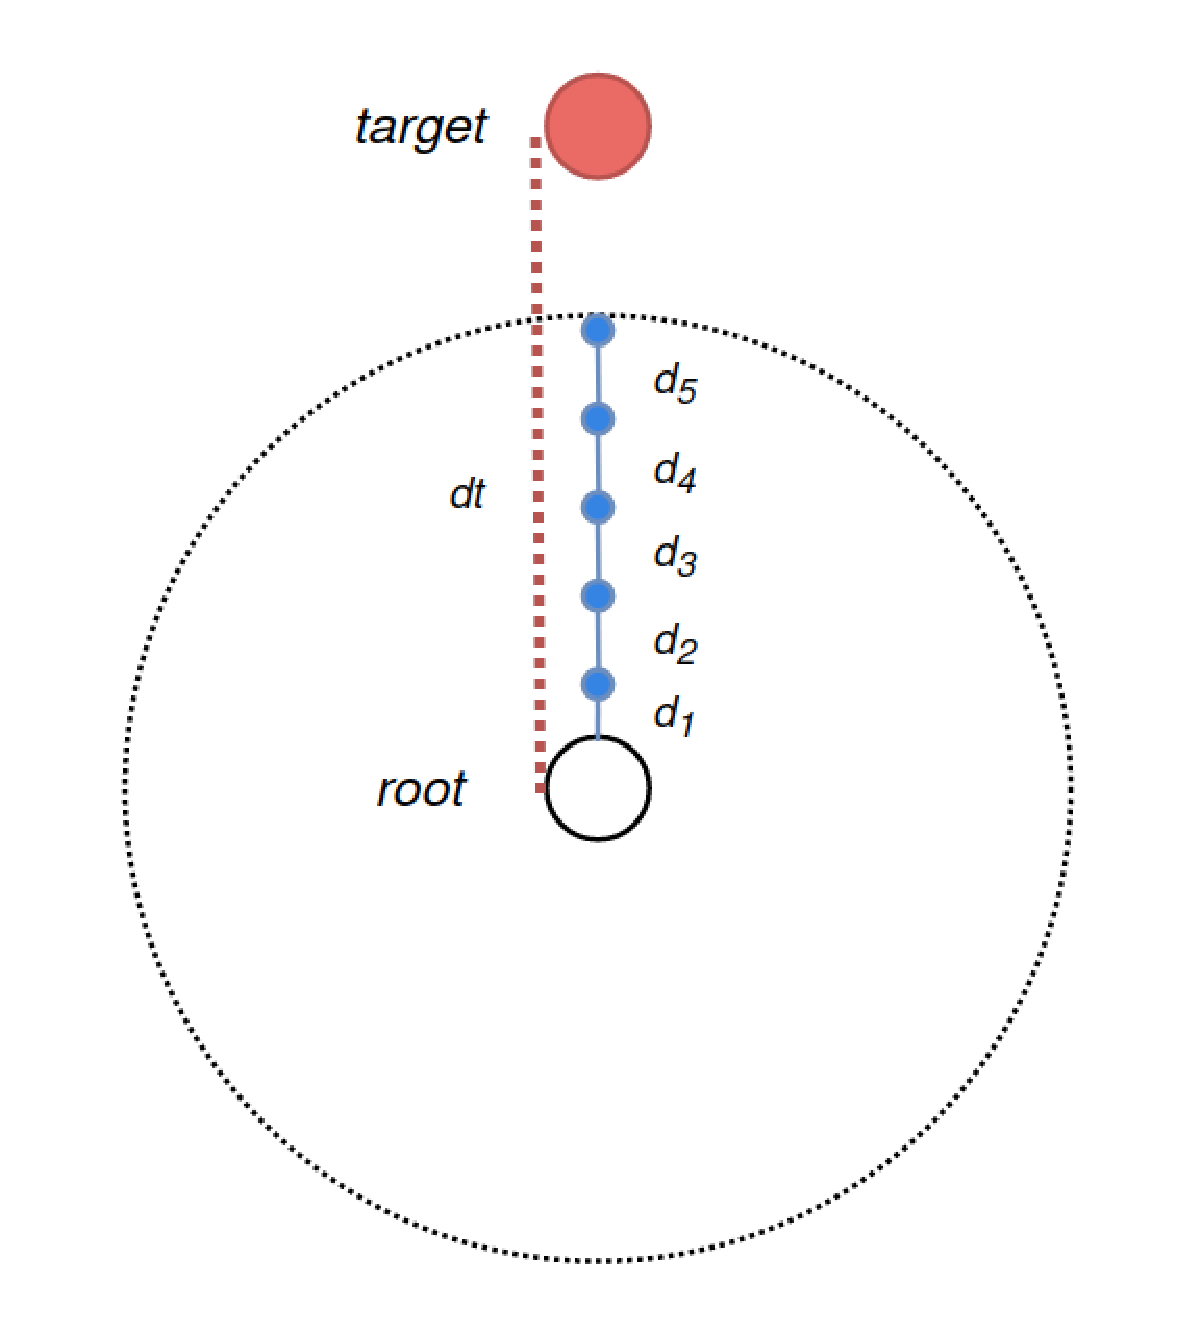
\includegraphics[width=0.5\textwidth]{grafika/unreachable_dist_1.eps}
    \caption{An IK problem with no solution where the target is unreachable
    because the sum of segment distances is less than the distance between the
    root and the target \(\sum_{i=1}^{n}d_i < dt\) }
    \label{fig:unreachable_dist1}
\end{figure}

\begin{figure}
    \centering
    \captionsetup{justification=centering}
    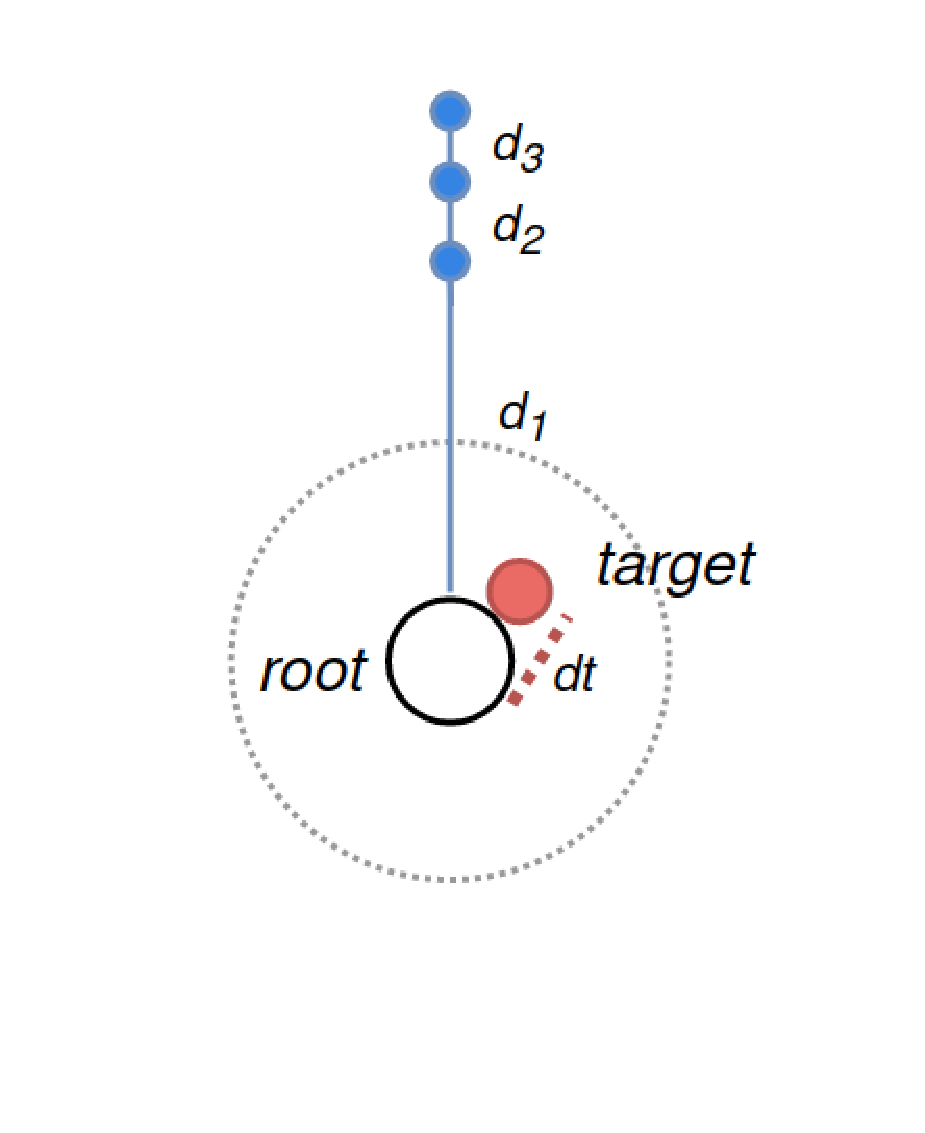
\includegraphics[width=0.4\textwidth]{grafika/unreachable_dist_2.eps}
    \caption{An IK problem with no solution where the target is unreachable
    because the length of the first segment is greater than the summed length of
    the rest of the kinematic chain \(d_1 - \sum_{i=2}^{n}d_i > dt\). This creates
    a radius around the root where if the root's distance to the target is
    smaller than the radius, the target is unreachable.
} \label{fig:unreachable_dist2}
\end{figure}

Another reason for the lack of solutions to an IK problem can be its
over-constraining. Constraints are used to dictate the range of motion of
each joint. For example, they might limit the joint's degrees of freedom by
reducing the dimensions in which it can perform its rotational and translational
transformations. They are often modelled after joints which are present in the
human body, such as hinge joints, ball joints, or pivot joints. A constraint can
also limit the extent of a joint's ability to bend which is defined by the
allowed angle of the joint's rotation in relation to the rotation of its parent
node. If too many of such constraints are added to a kinematic chain, it may
have blind spots for which it is unable to find a configuration of
transformations which can bend the chain to reach the target (Fig.
\ref{fig:unreachable_angles}).

\begin{figure}
    \centering
    \captionsetup{justification=centering}
    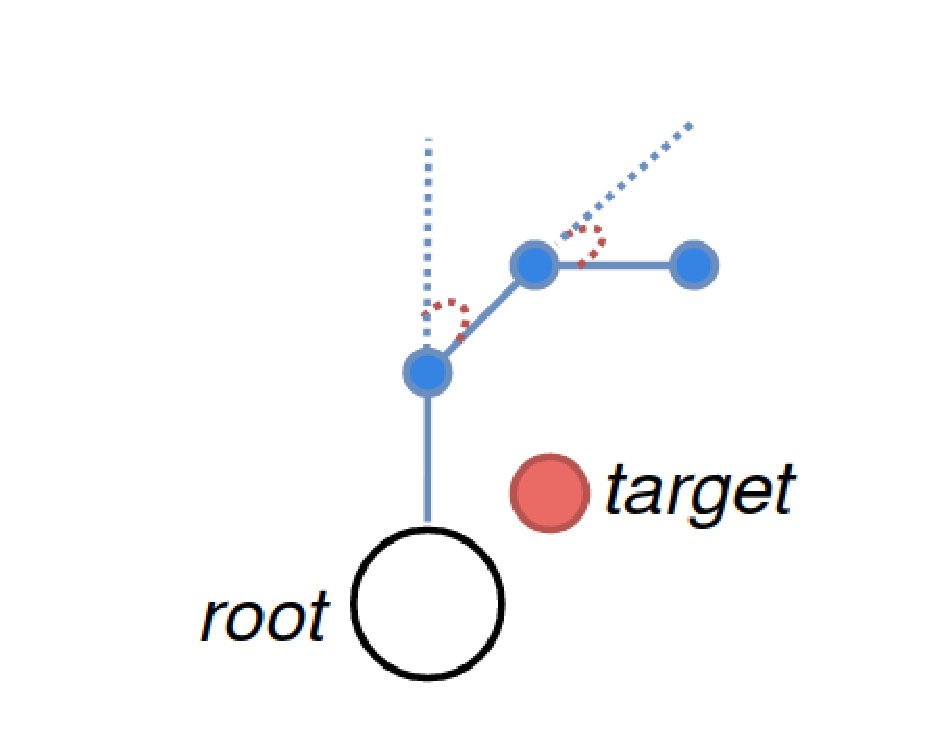
\includegraphics[width=0.4\textwidth]{grafika/unreachable_angles.eps}
    \caption{An IK problem with no solution where the rotational constraints
    placed on the joints prevent the end effector from being able to bend enough
    to reach the target}
    \label{fig:unreachable_angles}
\end{figure}

If a kinematic chain has more than one joint which is classified as an end
effector with its own separate target, a problem with no solutions can be
defined in a way that prevents both end effectors from reaching their target.
If at least one end effector is unable to reach its target then the problem can
be said to be unsolvable. \\

\noindent\textit{One or many solutions}

When an IK problem is not limited by the cases mentioned above, it can have one,
or many solutions depending on the case and constraints. More often than not the
problem will have multiple solutions, and if the kinematic chain is
unconstrained, the solution set for and IK problem grows very large.

While the introduction of constraints can decrease the number of solutions, the
simplest case to consider for an unconstrained kinematic chain is one where the
chain must stretch to its full extent in order to reach the target. The sum of
the chain's segment lengths \(d_i\) is equal to the distance from the root to
the target \(dt\):
\begin{equation}
    \sum_{i=1}^{n}d_i = dt.
\end{equation}

\section{Underlying principals}
In order to describe the configuration of a given kinematic chain, a set of
scalars \(\theta_1, \dots, \theta_n\) called \textit{joint angles} are defined
for each of the chain's \(n\) joints transforms. A set of \(k\) joint
positions \(\mathbf{s}_1, \dots, \mathbf{s}_k\) is defined for the end
effectors, where these positions are a function of the chain's configuration.
With the joint angles in the form of a column vector \(\bm{\theta} = (\theta_1,
\dots, \theta_n)^T\), and the end effectors as the vector \(\mathbf{s}
= (\mathbf{s}_1, \dots, \mathbf{s}_k)^T\), their relation can be expressed as:
\begin{equation} 
    \mathbf{s} = f(\bm{\theta}).
\end{equation}

The above equation \cite{Aristidou:2018:IK_survey} presents the FK problem where
the position of an end effector is calculated based on the given configuration
of the chain. To define the IK problem, a configuration of scalars must be found
based on the given final positions of the end effectors.
\begin{equation}
    \bm{\theta} = f^{-1}(\mathbf{s})
\end{equation}

The problem lies in inverting \(f\), as it is non-linear. Taking this into
account, along with the fact that an IK problem may have no solutions, one
solution, or many solutions, an approximation approach can be taken to solve
the problem efficiently. This can be achieved with iterative and heuristic
algorithms.

\section{IK Algorithms}
The methods discussed in this chapter are numerical, which means that
they take an iterative approach to achieve a solution. The numerical methods
can be divided into the \textit{Jacobian}, \textit{Newton}, and
\textit{Heuristic} categories. A comprehensive review of these methods is given
by Aristidou and co-workers in \cite{Aristidou:2018:IK_survey}. For convenience,
the overview of these methods will follow their work.

\subsection{Jacobian methods}
This approach to the IK problem \cite{BALESTRINO19842435, wolovich, Baillieul} offers
a linear approximation through an iterative calculation which estimates a change
to the given configuration of joint scalars necessary to reduce the distance
between an end effector and its desired destination. This is done through the
use of a matrix \(J\) called the Jacobian matrix which contains partial
derivatives of the entire kinematic chain relative to the set of end effectors.
\(J\) is a function of the chain configuration's joint angle scalars:
\begin{equation}
    J(\bm{\theta})_{ij} = \left(\frac{\partial s_i}{\partial
    \theta_j}\right)_{ij}
\end{equation}

\noindent as provided by \cite{rbuss_ik_survey}, where \(n\) and \(k\) are the
previously defined number of joints and number of end effectors in the chain
respectively. Given the position \(\mathbf{p}_j\) of the \(j\)th joint and its
current rotational axis \(\mathbf{v}_j\), each entry of the Jacobian matrix can
be defined by the cross product
\begin{equation}
    \frac{\partial s_i}{\partial \theta_j} = \mathbf{v}_j \times (\mathbf{s}_i
    - \mathbf{p}_j).
\end{equation}

With prime notation denoting a first derivative with respect to time, the
forward dynamics equation can be written as
\begin{equation}
    \mathbf{s}^\prime = J\bm{\theta}^\prime.
\end{equation}

A change to the kinematic chain's configuration \(\Delta \bm{\theta}\) is then
needed, which when applied, updates the end effectors to minimize their distance
to the targets. The resulting change in the end effector positions \(\Delta
\mathbf{s}\) due to the modification of the configuration is then approximated
as
\begin{equation}
    \Delta \mathbf{s} \approx J \Delta \bm{\theta},
    \label{eqn:fk_approx}
\end{equation}

\noindent and the changes made to the joint scalars should be done in a way
where the change in end effector positions \(\Delta\mathbf{s}\) minimizes the
error \(\mathbf{e}\), which is a vector of changes in position required for each
of the chain's end effectors to reach their desired positions. Supposing that
\(\mathbf{t}_i\) is the target position for the end effector \(i\), the errors
can be defined as \(\mathbf{e}_i = \mathbf{t}_i - \mathbf{s}_i\). By applying a left
matrix multiplication by \(J^{-1}\) to both sides of (\ref{eqn:fk_approx}), the
IK problem for the Jacobian method is rewritten as follows: 
\begin{equation} 
    \Delta \theta \approx J^{-1}\mathbf{e},
\end{equation}
\noindent where \(\Delta\mathbf{s}\) is substituted by \(\mathbf{e}\) due to
them being approximately equal to each other.

A solution to this Jacobian method of the IK problem is not always simple due to
the possibility of a non-invertible matrix, or singularities which prevent
changes of the chain's configurations which achieve the sought-after result in
end effector positions. Certain methods have been brought forward to surmount
these challenges. \\

\noindent\textit{Pseudo-Inverse}

To address the problem of non-invertible Jacobian matrices, the Jacobian
Pseudo-inverse \(J^\dagger\), also called the \textit{Moore-Penrose inverse}
\cite{golub_matrix3} can be used as
a substitute:
\begin{equation}
    \Delta \theta = J^{\dagger}\mathbf{e}
\end{equation}
The benefit of using the pseudo-inverse method is that the matrix \(J^\dagger\)
is defined for every case of the Jacobian matrix, whether it is invertible or
not. The pseudo-inverse matrix is defined as
\begin{equation}
    J^\dagger = J^T (J J^T)^{-1}
\end{equation}

Where the pseudo-inverse falls short is when approaching singularities. In these
cases, the resulting values become unstable leading to oscillations. \\

\noindent\textit{Jacobian Transpose}

Another way to overcome the case where \(J\) is a non-invertible matrix is to
use the matrix transpose instead. An so, the inverse is substituted with the
transpose, with a coefficient \(\alpha\):
\begin{equation}
    \Delta \theta = \alpha J^T \mathbf{e}.
\end{equation}

In order to minimize the distance of each \(\mathbf{e}\) between  the end effectors and
their targets, the coefficient \(\alpha\) is calculated with the goal of
achieving the smallest value of \(\mathbf{e}\) after each iteration. The equation
which models this calculation is as follows

\begin{equation}
    \alpha = \frac
        {
            \langle\mathbf{e}, J J^T \pvec{e}\rangle
        }
        {
            \langle J J^T \mathbf{e},J J^T \pvec{e} \rangle
        }
\end{equation}

\noindent where the angular brackets represent a dot product operation between the two
values contained inside them. The value of the coefficient \(\alpha\) must be
small enough to avoid oscillations, and due to this the process of converging
end effectors on the targets is slow and requires many iterations to achieve
a desired configuration. \\

\noindent\textit{Other Jacobian methods}

A multitude of approaches to the IK problem using Jacobian methods have been
suggested, some of which are variations or combinations of the presented
methods. Among others, the Singular Value Decomposition method \cite{num_recipes}
extends the pseudo-inverse method with orthogonal matrices, the Damped
Least Squares method \cite{Wampler1986ManipulatorIK} helps avoid problems with
singularities present in the pseudo-inverse method, the Pseudo-inverse Damped
Least Squares method \cite{maciejewski, num_recipes} combines the two previously
mentioned methods to improve their instability when nearing singularities, and
the Selectively Damped Lease Squares method \cite{buss_kim_sdls} builds on the
previous method to converge in fewer iterations and optimize for multiple end
effectors. A deep-learning approach to the Damped Lease Squares method was also
proposed \cite{wang_dldls} with the aim of predicting the most optimal value for
certain coefficients.

\subsection{Newton Methods}
The Newton methods are based on a second order Taylor series expansion of the
function \(f(x)\) with \(H_f(x)\) being the Hessian matrix:
\begin{equation}
    f(x + \sigma) \approx f(x) + |\nabla f(x)|^T \sigma + \frac{1}{2} \sigma^T H_f(x)
    \sigma
\end{equation}

The Newton methods have the advantage over the Jacobian inverse methods in the
smoothness of the movement and the lack of singularity problems which allows the
iterative approach to avoid oscillations. However, the complexity of the Hessian
matrix drastically raises the computational costs for each iteration. A few
methods have been brought forward which aim to approximate the Hessian matrix
to reduce the complexity of the problem, however the computational costs remain
relatively high.

\subsection{Heuristic IK algorithms}
Heuristic algorithms provide an approach which avoid the need for complex
equations and heavy computations, and instead act as techniques to achieve an
approximate solution iteratively in a much more simple way. These methods are
very popular in the domain of computer graphics and animation, due to the
problems not needing extremely accurate solutions but benefiting from a simple
and fast approach in the real-time environment of video games. \\

\noindent\textit{Cyclic Coordinate Descent}

The Cyclic Coordinate Descent (CCD) algorithm \cite{ccd} is one of the simplest and most
used IK solutions in the computer games industry. It also finds
applications in robotics as well as the already mentioned protein structure
prediction \cite{ccd_protein}. 

The algorithm acts on each joint transform separately, minimizing the distance
between the end effector and the target by finding the appropriate angle by
which it should rotate the given joint. The iteration begins at the end of the
chain, excluding the end effector. The desired angle of rotation is calculated by
finding lines, one of which passes through the current joint and the end
effector, while the other passes through the current joint and the target. The
angle between these two lines is the angle by which the current joint should
be rotated in order to place the end effector on the line spanning between the
current joint and the target, thus reducing the distance between the end
effector and the target as much as possible (Fig. \ref{fig:ccd}). The
algorithm is repeated iteratively until the distance between the end effector
and the target is smaller than some threshold.

\begin{figure}
    \centering
    \captionsetup{justification=centering}
    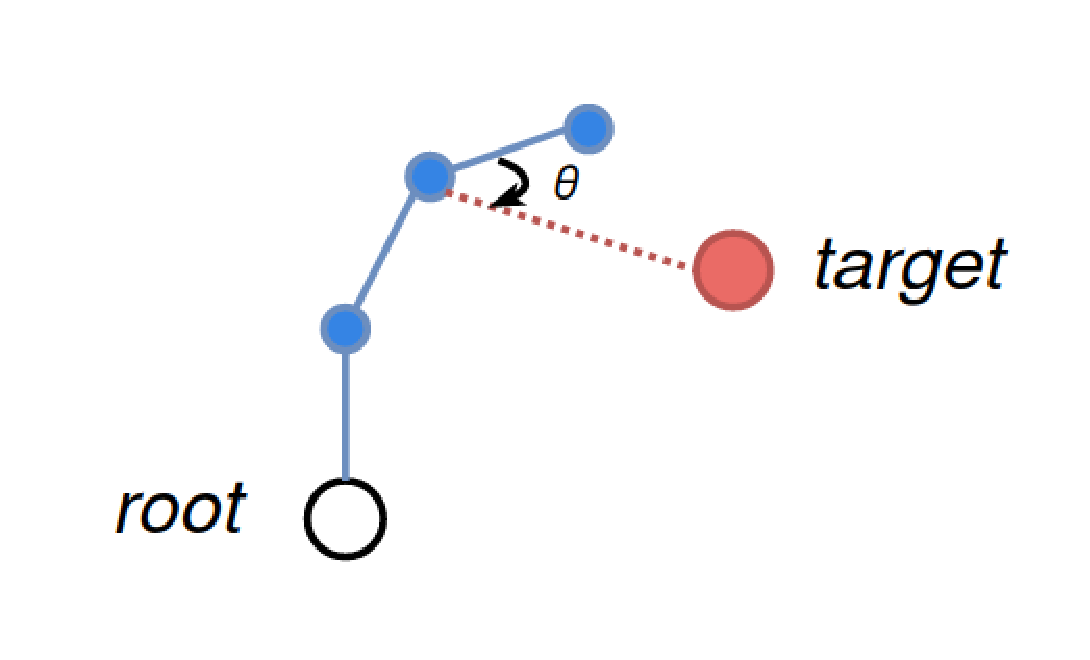
\includegraphics[width=0.4\textwidth]{grafika/ccd_1}
    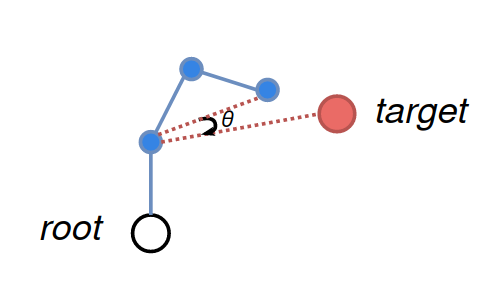
\includegraphics[width=0.4\textwidth]{grafika/ccd_2}
    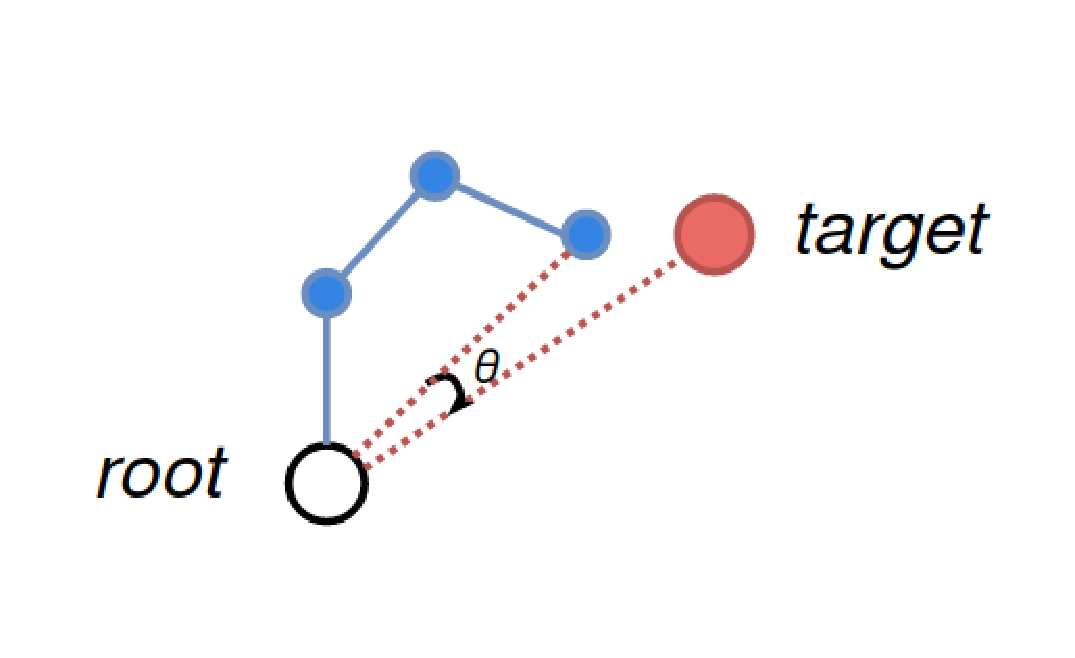
\includegraphics[width=0.4\textwidth]{grafika/ccd_3}
    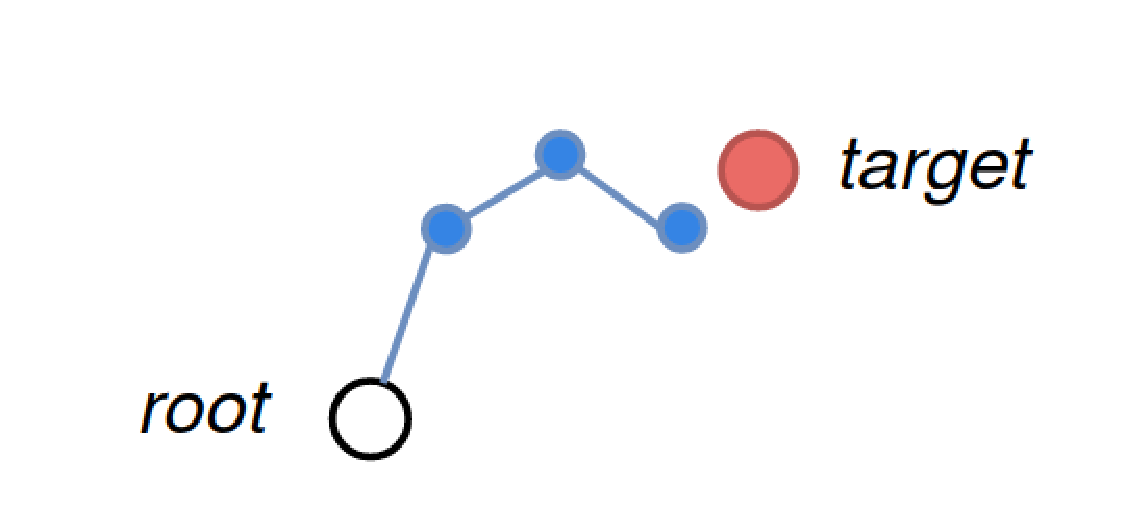
\includegraphics[width=0.4\textwidth]{grafika/ccd_4}
    \caption{A single pass of the CCD algorithm}
    \label{fig:ccd}
\end{figure}

While the CCD algorithm is very fast and simple to implement, it often produces
unrealistic movements and unnatural poses when applied to a kinematic chain,
partly due to the fact that the joints closer to the end effector have a high
impact on the resolution of the problem, and the joints further away have
a smaller impact. The unequal distribution of adjustments in the chain's
configuration lead to chaotic animations. The algorithm also has a lesser
affinity for solving IK problems with multiple end effectors, and to overcome
this, a system with multiple end effectors must first be broken down into
independent chains. \\

\noindent\textit{Forward and Backward Reaching Inverse Kinematics}

The Forward and Backward Reaching Inverse Kinematics (FABRIK) algorithm
\cite{Aristidou2011} is another heuristic approach to the IK problem which
gained popularity in computer graphics and video games. 

Like the CCD algorithm, FABRIK iterates over the joints of a kinematic chain,
adjusting them one at a time. However, this algorithm involves two passes per
iteration where, as the name suggests, one pass is done starting from the end
effector iterating towards the root, while the second pass is done in a reversed
order as shown in Fig. \ref{fig:fabrik}. The algorithm starts by checking if the
target is in reach before proceeding to iterate over the kinematic chain. 

\begin{figure}[!h]
    \centering
    \captionsetup{justification=centering}
    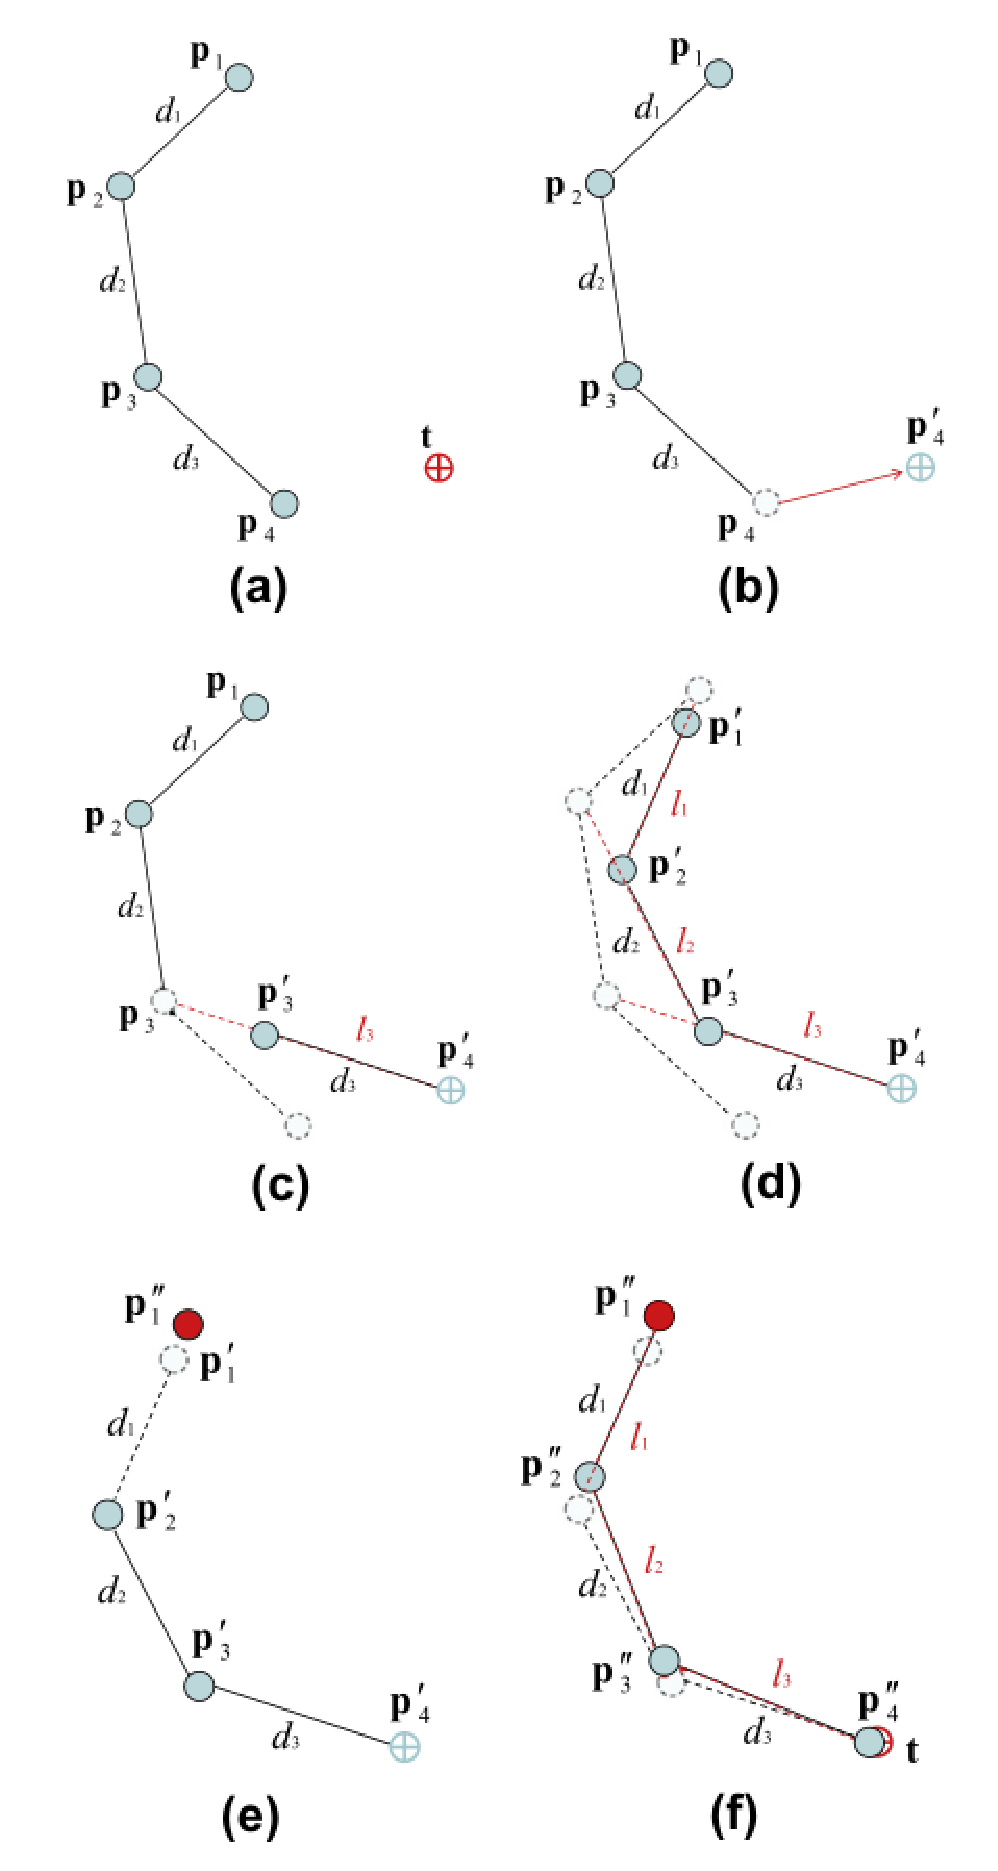
\includegraphics[width=0.4\textwidth]{grafika/fabrik_iteration.eps}
    \caption{An iteration of the FABRIK algorithm where (a) through (d) are
    detailed steps of the forward pass while (e) and (f) show the solution of
    the backward pass. Source: \cite{Aristidou2011}}
    \label{fig:fabrik}
\end{figure}

For a set of \(n\) joint positions \(\mathbf{p}_1, \dots, \mathbf{p}_n\) where
\(\mathbf{p}_1\) is the root and \(\mathbf{p}_n\) is the end effector, the forward pass
begins by setting the position of the end effector to that of the target. The
next joint \(\mathbf{p}_{n-1}\) is then linearly interpolated on a line which
passes through its current position and the position of the previously affected
joint, in this case, the end effector. The interpolation is done to preserve the
distance between the joints. Thus, the forward pass of the algorithm can be
modeled by 
\begin{equation}
    \mathbf{p}_i = (1 - \lambda_i)\mathbf{p}_{i+1} + \lambda_i \mathbf{p}_i,
\end{equation}

\noindent where \(\lambda_i\) is a coefficient which ensures that the linear interpolation
preserves the distance between joint positions \(\mathbf{p}_i\) and
\(\mathbf{p}_{i+1}\). When the forward pass is finished, the root ends up being
displaced from its original position, and in order to rectify this a backwards
pass is initiated in a reverse order which starts by setting the root back to
its original position. The iteration proceeds very similarly to the forwards
pass, this time interpolating each joint \(\mathbf{p}_i\) between its current
position and the new position of \(\mathbf{p}_{i-1}\). The backwards pass is then
\begin{equation}
    \mathbf{p}_i = (1 - \lambda_i)\mathbf{p}_{i-1} + \lambda_i \mathbf{p}_i.
\end{equation}

The iterations are repeated until the distance between the end effector and the
target are smaller than some threshold, at which point the problem can be
considered solved.

The FABRIK algorithm is very fast due to its calculations relying on adjusting
positions along a line instead of calculating joint angles. This also majorly
simplifies its implementation. It also provides a more natural configuration as
a solution to the IK problems compared to the CCD algorithm as the degree to
which each joint is adjusted during the iterations is not unevenly distributed
along the chain. Additionally, the FABRIK algorithm is a good fit for computer
graphics and animation because of its ability to handle multiple end effectors
well and to be constrained in multiple ways.

For the purpose of this paper, the FABRIK algorithm was chosen as the
algorithm to be implemented in the demo application. The choice helps avoid the
problems with singularities which exist when using the Jacobian methods, the
complex implementations and heavy calculations of the Newton methods, and
instead provides a fast and lightweight algorithm which is simple to implement
and has a better chance of producing more natural kinematic chain configurations
than the CCD algorithm. The FABRIK algorithm also finds its implementations in
many software programs, including the built-in Unity \textit{Animation Rigging}
package \cite{unity_animation_rigging}.

